\section{Variational Analysis} \label{sec:variational}

We performed two analyses to characterize the properties of our five match distance metrics under bitwise mutation.
Single-step mutational analysis examines the local mutational neighborhood of tag pairs.
Then, mutational walk analysis surveys the topography of the wider mutational landscape.

\subsection{Single-Step Mutations}

\begin{figure}
\begin{center}

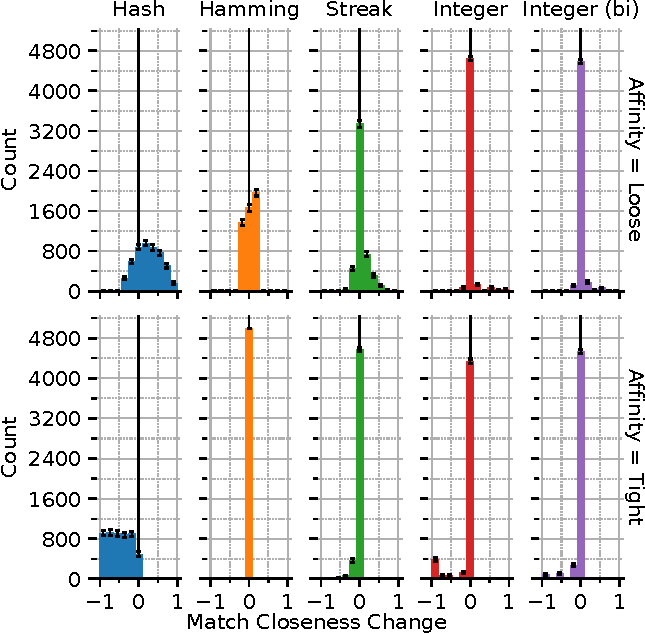
\includegraphics[width=\columnwidth]{img/mutational_step/bitweight=0dot5+seed=1+title=low-mutational-step+viz=hist+_data_hathash_hash=95a57768de56995a+_script_fullcat_hash=aa068ad24b386169+ext=}
\caption{
Distributions of mutation effects on match distance for loosely matched (pre-mutation match distance $> 0.5$) and tightly matched (pre-mutation match distance $< 0.01$) tag pairs.
Note that match closeness change (rather than mast distance change) is plotted so that better-matching mutational outcomes fall to the right and worse-matching mutational outcomes fall to the left.
Error bars are 95\% confidence intervals calculated using the Wilson score method with continuity correction \citep{newcombe1998two}.
Supplementary Figure \ref{fig:mutational_step_supp} shows the cumulative distribution of all sampled match distance changes for each metric.
}
\label{fig:mutational_step}

\end{center}
\end{figure}


Figure \ref{fig:mutational_step} visualizes the distribution of match distance outcomes of single-bit mutations.
We provide this analysis for two categories of tag pairs: tags that were loosely affiliated and tags that were tightly affiliated.

To measure the distribution of mutational perturbations on loosely-affiliated tag pairs we began by sampling a target tag and then randomly sampled candidate tags until we found a second tag with a match distance $> 0.5$.
We recorded the match distance between our tag pair, applied a one-bit mutation to the secondary tag, and then measured the match distance between the tag pair again.
Mutational perturbation was calculated as the difference between the match distances.
A negative mutational perturbation indicates a decrease in match distance and, therefore, an increase in match quality.

We measured the distribution of mutational perturbations on tightly-matched tag pairs similarly, except we uniformly sampled secondary candidate tags until we found a second tag with match distance $< 0.01$.
We sampled 5000 tightly-matched measurements and 5000 loosely-matched measurements for each metric.

For both tightly- and loosely-affiliated tag pairs under the integer and bidirectional integer metrics, most mutations caued very small changes in match distance.
These mutations likely the toggle least-significant bits of the tag's integer representation.
However, under these metrics, a small fraction of mutations affecting more-significant bits of the integer representation have a much stronger effect.
Single-step mutations occassionally occur that strongly couple loosely-affiliated tag pairs or strongly decouple tightly-affiliated tag pairs.
In particular, the unidirectional integer metric, presumably due to its non-commutative quirks, appers to exhibit more frequent strong decoupling mutations than the bidirectional integer metric.

The streak metric is the only metric that exhibits perfectly neutral outcomes under mutation.
These perfectly-neutral mutations presumably affect regions of the bitstring involved neither in the longest-matching streak nor in the longest-mismatching streak.
The streak metric appears to exhibit a fatter tail of match-distance magnitude for mutations that couple loosely-affiliated tags than the integer metrics.
In addition, the most extreme mutational outcomes that couple loosely-affiliated tags appear to be of a comparable magnitude to those under the integer metrics.
Mechanistcally, this might be due to mutations that disrupt longest-mismatching streaks.
However, one-step mutations that decouple tightly-affiliated tags do not appear as potent.
This might be because achieving a very poor match requires both increasing longest-mistmatching streak length and decreasing longest-matching streak length.

The hamming metric exhibits a generally uniform magnitude of match-distance changes under mutation.
High-magnitude one-step mutations do not occur under this metric.
(Without normalizing match distance to a uniform distribution for randomly-sampled tags, all hamming metric mutations would be of exactly the same magnitude, either increasing or decreasing the count of matching bits by 1).

The hash metric exhibits the fattest tails of mutational magnitude of all metrics.
Extreme-effect one-step mutations are plentiful under this metric.
Interestingly, compared to other metrics, the hash metric exhibits a greater fraction of mutations that decouple tightly-affiliated tags and a greater fraction of mutations that coouple loosely-affiliated tags.
This might be due to the hash metric's lack of geometric structure.
Because all one-step mutations uniformly sample a new match distance, 99\% of one-step mutations on tightly-affiliated tags will result in a looser coupling.
Similarly, approximately 75\% of one-step mutations on loosely-affiliated tags will result in a tigher coupling.

\subsection{Mutational Walks}

\begin{figure*}
\begin{center}

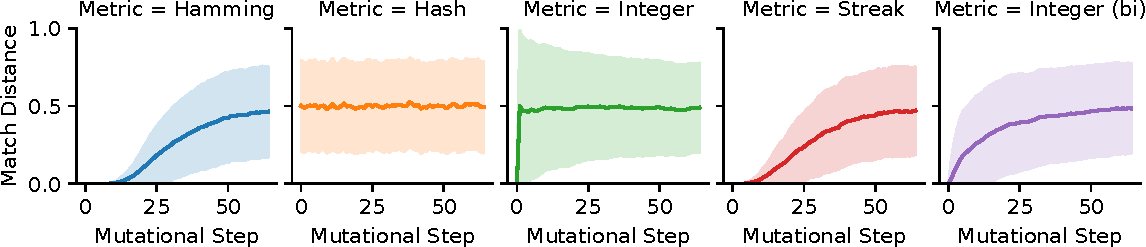
\includegraphics[width=\textwidth]{{{mutational_walk/bitweight=0.5+seed=1+title=mutational_walk_lineplot+_data_hathash_hash=ff15c8831d4f9288+_script_fullcat_hash=c872df869f05035a+ext=}}}
\caption{
TODO
}
\label{fig:mutational_walk_lineplot}

\end{center}
\end{figure*}

\begin{figure}
\begin{center}

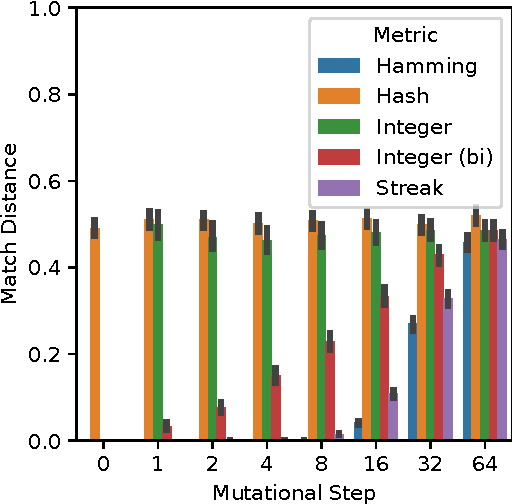
\includegraphics[width=\columnwidth]{{{mutational_walk/bitweight=0.5+seed=1+title=mutational_walk_barplot+_data_hathash_hash=8bf152d87daa9cb7+_script_fullcat_hash=982405ca713eba73+ext=}}}
\caption{
Snapshots of match distance at exponentially increasing steps from identical tags.
Error bars represent 95\% confidence intervals.
}
\label{fig:mutational_walk_barplot}

\end{center}
\end{figure}


Next, we performed mutational walks under each metric.
We began with two randomly chosen equivalent tags (mutation step zero) then applied randomly chosen one-step mutations (with the possibility of back mutation allowed) 65 times to the second tag.
We measured match distance between the two tags at each mutational step.
We performed 1000 independent mutational walks from different starting equivalent tags.

Figure \ref{fig:mutational_walk_lineplot} continuously depicts the distribution of match distances on mutational walks, with shaded areas indicating standard deviation, under different metrics.
Figure \ref{fig:mutational_walk_barplot} compares match distances at exponentially increasing steps.
Error bars indicate 95\% confidence intervals.

For the hash metric, where equivalent tags don't necessarily have low match distance, the mutational walk wanders around loose affinity.

The Spector Integer metric, where half of mutational steps wrap back around to 1.0 distance, immediately spikes up to an average match distance of 0.5.
The variance decreases with mutational steps as the distribution moves away from bias towards distances of 0 and 1.

The bidirectional integer metric experiences a greater immediate jump in variance and significantly greater mean match distance as rare mutations affecting significant bits take place (non-overlapping 95\% CI).

The
Intrestingly, contrary to as was claimed in \citep{downing2015intelligence}, the uniformified streak metric's match score under mutation actually grows significantly faster than the hamming metric's match score  (non-overlapping 95\% CI).

Because the are uniformified, the distributions all devolve to having an equivalent mean and variance.


